% =============================================================================
% Paper 1: Soft-Exp Inference for Autoregressive LM
% Target: ICLR Workshop / ACL Findings / arXiv
% Format: NeurIPS-style (4 pages main + unlimited appendix)
% =============================================================================
\documentclass{article}

% NeurIPS-style packages
\usepackage[preprint]{neurips_2024}
\usepackage[utf8]{inputenc}
\usepackage[T1]{fontenc}
\usepackage{hyperref}
\usepackage{url}
\usepackage{booktabs}
\usepackage{amsfonts}
\usepackage{nicefrac}
\usepackage{microtype}
\usepackage{xcolor}
\usepackage{amsmath}
\usepackage{graphicx}
\usepackage{algorithm}
\usepackage{algorithmic}
\usepackage{listings}

% For author names and affiliations
\title{Exposure Bias is Bigger Than You Think:\\
       Continuous Expected Embeddings as a Drop-In Fix for Autoregressive Decoding}

\author{%
  Yiming Wang \\
  CrystaLLM Project \\
  \texttt{yiming.wang@crystallm.org} \\
}

\begin{document}

\maketitle

\begin{abstract}
Autoregressive language models are trained with teacher forcing but deployed by feeding back their own discrete predictions, creating a structural train-inference mismatch. We measure this gap on a 1.2B-parameter Transformer: teacher-forcing perplexity is 3.26, but standard argmax-feedback inference yields 64.74---a $19.88\times$ degradation, far larger than the $\sim 1.1\times$ commonly cited in textbooks. We propose \textbf{Soft-Exp inference}: replace the discrete argmax token embedding with the continuous probability-weighted expected embedding. This single-line change (no retraining, no architectural modification) reduces inference perplexity to 33.27, halving the exposure bias ($+48.6\%$ relative improvement). The improvement is \emph{scale-invariant}: at 2M, 8M, 16M, and 1.2B parameters, Soft-Exp yields $+81\%$, $+53\%$, $+48.6\%$, and $+48.6\%$ respectively. Soft-Exp is the inference-time dual of scheduled sampling \citep{bengio2015scheduled}: both target the train-inference mismatch from opposite sides, and we show that Soft-Exp achieves the goal without destabilizing training. We discuss why continuous feedback preserves more distributional information than discrete point estimates, and connect the result to soft-target distillation \citep{hinton2015distill}.
\end{abstract}

% =============================================================================
\section{Introduction}
% =============================================================================

Autoregressive language models are trained to predict $p_\theta(x_t \mid x_{<t})$ under teacher forcing: at each position, the model sees ground-truth context and is graded on the next token's cross-entropy. At inference, the model is rolled out autoregressively, feeding back its own predictions.

This train-inference gap is known as \emph{exposure bias} \citep{bengio2015scheduled}. The standard framing emphasizes that the model's input distribution at inference differs from training: at training, every position sees ground-truth context; at inference, every position sees model-generated context (which may contain errors that compound).

We measure the magnitude of this gap empirically on a 1.2B-parameter Transformer trained on char-level text. With identical model weights:
\begin{itemize}
    \item \textbf{Teacher forcing} PPL: $3.26$ (oracle capacity, no distribution shift)
    \item \textbf{Argmax feedback} PPL: $64.74$ ($19.88\times$ degradation)
\end{itemize}

This $20\times$ gap is not a corner case---it is the operating regime of every autoregressive LM in production. It is also much larger than the $\sim 1.1\times$ gap suggested by typical textbook treatments.

\paragraph{The fix.} We propose \textbf{Soft-Exp inference}: at each step, instead of feeding back the embedding of the argmax token (a discrete point estimate), feed back the \emph{continuous expected embedding}, the probability-weighted sum of all token embeddings:
\begin{align*}
    \mathbf{e}_{\text{next}} &= \mathbf{p}^\top \mathbf{E} \quad \text{where } \mathbf{p} = \mathrm{softmax}(\mathbf{z}_t),\ \mathbf{E} \in \mathbb{R}^{V \times d}
\end{align*}

This is a one-line code change:
\begin{lstlisting}[language=Python]
# Standard AR inference:
next_embed = token_emb(argmax(logits))

# Soft-Exp inference:
next_embed = probs @ token_emb.weight  # 1 line
\end{lstlisting}

On V49 1.2B, Soft-Exp reduces inference PPL to $33.27$---a $+48.6\%$ relative improvement over argmax, halving the exposure bias to $10.22\times$.

\paragraph{Scale invariance.} We validate Soft-Exp across four model scales (2M, 8M, 16M, 1.2B parameters). The relative improvement is approximately constant across this $600\times$ parameter range:
\begin{center}
\small
\begin{tabular}{lcccc}
\toprule
Scale & 2M & 8M & 16M & 1.2B \\
\midrule
Soft-Advantage & $+81\%$ & $+53\%$ & $+48.6\%$ & $+48.6\%$ \\
\bottomrule
\end{tabular}
\end{center}

The improvement does \emph{not} grow with scale, suggesting it is a property of the inference scheme, not a small-model artifact.

\paragraph{Contributions.}
\begin{enumerate}
    \item Empirical quantification of exposure bias at $1.2$B scale: a $19.88\times$ gap.
    \item A drop-in inference fix: Soft-Exp, one line of code, no retraining.
    \item Scale-invariant validation across 600$\times$ parameter range.
    \item Connection to soft-target distillation and theoretical analysis of why continuous feedback preserves more information than discrete point estimates.
\end{enumerate}

\paragraph{What this paper is not.} We do not eliminate exposure bias---Soft-Exp reduces it from $19.88\times$ to $10.22\times$. The residual gap is structural; closing it requires changes to the training procedure, which we explore and reject in companion work \citep{wang2026failed}.

% =============================================================================
\section{Background}
% =============================================================================

\subsection{Autoregressive LM training and inference}

Given a sequence $x_1, \ldots, x_T$, an AR model computes $p_\theta(x_t \mid x_{<t})$ for each position. Training minimizes cross-entropy:
\begin{align*}
    \mathcal{L}_\text{TF} = -\sum_t \log p_\theta(x_t \mid x_{<t})
\end{align*}
with teacher-forced inputs $x_{<t}$. At inference, the model rolls out autoregressively:
\begin{align*}
    \hat{x}_t &= \mathrm{argmax}\ p_\theta(\cdot \mid \hat{x}_{<t}) \\
    \mathbf{h}_t &= f_\theta(\mathbf{h}_{t-1}, \mathrm{emb}(\hat{x}_{t-1}))
\end{align*}

The mismatch between $\mathrm{emb}(x_{t-1})$ at training (ground truth) and $\mathrm{emb}(\hat{x}_{t-1})$ at inference (model prediction) is the source of exposure bias.

\subsection{Prior work: scheduled sampling}

\citet{bengio2015scheduled} introduced \emph{scheduled sampling}: during training, occasionally replace ground-truth input with the model's own prediction. This bridges the train-inference gap but introduces its own problems:
\begin{itemize}
    \item The training loss becomes noisier (mixed objective)
    \item The model sees inconsistent training signal
    \item The expected inference distribution still differs from training
\end{itemize}

\citet{huszar2015how} showed that scheduled sampling implicitly optimizes a different objective than maximum likelihood, and proposed alternatives that retain the MLE property.

\subsection{Soft targets and knowledge distillation}

\citet{hinton2015distill} showed that training on \emph{soft targets} (probability distributions over classes) carries more information per example than hard one-hot targets. The principle: a soft target retains the model's uncertainty about the correct answer, which is informative about class similarity.

Our key observation: \emph{at inference time, the model's own predicted distribution is a soft target}. Feeding back the expected embedding under this distribution (rather than its mode) is the inference-time analog of training on soft targets.

% =============================================================================
\section{Method: Soft-Exp Inference}
% =============================================================================

\subsection{Definition}

Standard AR decoding computes, at each step $t$:
\begin{align*}
    \mathbf{z}_t &= \mathrm{head}(f_\theta(\mathbf{h}_{t-1}, \mathrm{emb}(\hat{x}_{t-1}))) \\
    \hat{x}_t &= \mathrm{argmax}\ \mathrm{softmax}(\mathbf{z}_t)
\end{align*}
and feeds back $\mathrm{emb}(\hat{x}_t)$.

\textbf{Soft-Exp decoding} replaces the discrete feedback:
\begin{align*}
    \mathbf{e}_t &= \mathbf{p}_t^\top \mathbf{E} \quad \text{where } \mathbf{p}_t = \mathrm{softmax}(\mathbf{z}_t) \\
    \mathbf{h}_t &= f_\theta(\mathbf{h}_{t-1}, \mathbf{e}_t)
\end{align*}

The expectation $\mathbf{e}_t$ is a continuous point in the embedding space, lying in the convex hull of $\{\mathrm{emb}(v) : v \in \mathcal{V}\}$.

\subsection{Computational cost}

Per inference step, Soft-Exp adds:
\begin{itemize}
    \item One $\mathrm{softmax}$ over the vocabulary ($\mathcal{O}(V)$)
    \item One matmul of probability vector $\times$ embedding matrix ($\mathcal{O}(V \cdot d)$)
\end{itemize}
This is negligible compared to the Transformer forward pass ($\mathcal{O}(L \cdot d^2 \cdot T)$). We measured no measurable throughput difference between argmax and Soft-Exp decoding.

\subsection{Why it works: information-theoretic view}

Argmax is the 0-th order statistic of the predictive distribution: only the mode is retained, all uncertainty is discarded.

Soft-Exp (the expected embedding) is the 1st order statistic: the mean embedding under $p_\theta(\cdot \mid \hat{x}_{<t})$ is retained. This preserves the model's uncertainty about the next token, encoded as a continuous point in the embedding manifold.

By analogy with knowledge distillation, the dark knowledge (non-maximal probabilities) carries information about class similarity that the hard target discards. We argue similarly: the dark knowledge in the predictive distribution carries information about the embedding manifold's local geometry that the discrete point estimate discards.

% =============================================================================
\section{Experiments}
% =============================================================================

\subsection{Setup}

\paragraph{Model.} V49 baseline Transformer (Pre-LN, learned positional embeddings, GELU MLP), identical architecture as \citet{v49scale}. Char-level vocabulary ($V=2261$), sequence length 128.

\paragraph{Scales.} 2M, 8M, 16M, 32M, and 1.2B parameters. All trained on the same corpus subset (v28, $\sim$65M tokens) with identical hyperparameters except width and depth. Training: AdamW, peak LR $5 \times 10^{-5}$, 1000-step warmup, cosine decay.

\paragraph{Evaluation.} We compare three decoding modes:
\begin{itemize}
    \item \textbf{Teacher Forcing (TF)}: oracle input, measures model capacity.
    \item \textbf{Argmax}: standard AR inference, baseline.
    \item \textbf{Soft-Exp}: continuous expected embedding feedback.
\end{itemize}
We report validation perplexity on the held-out set. For autoregressive modes, we use sequence length 64 and 50 sequences per evaluation batch.

\subsection{Main result: V49 1.2B}

\begin{table}[h]
\centering
\small
\begin{tabular}{lccc}
\toprule
Mode & Val PPL & $\times$ TF & Notes \\
\midrule
Teacher Forcing & $3.26$ & $1.00\times$ & oracle upper bound \\
Argmax          & $64.74$ & $\mathbf{19.88\times}$ & standard AR inference \\
Soft-Exp        & $\mathbf{33.27}$ & $\mathbf{10.22\times}$ & \textbf{ours, +48.6\% vs argmax} \\
\bottomrule
\end{tabular}
\caption{V49 1.2B three-mode validation perplexity. Soft-Exp cuts exposure bias in half.}
\label{tab:main}
\end{table}

Figure~\ref{fig:main} visualizes the gap and the Soft-Exp improvement.

\begin{figure}[h]
\centering
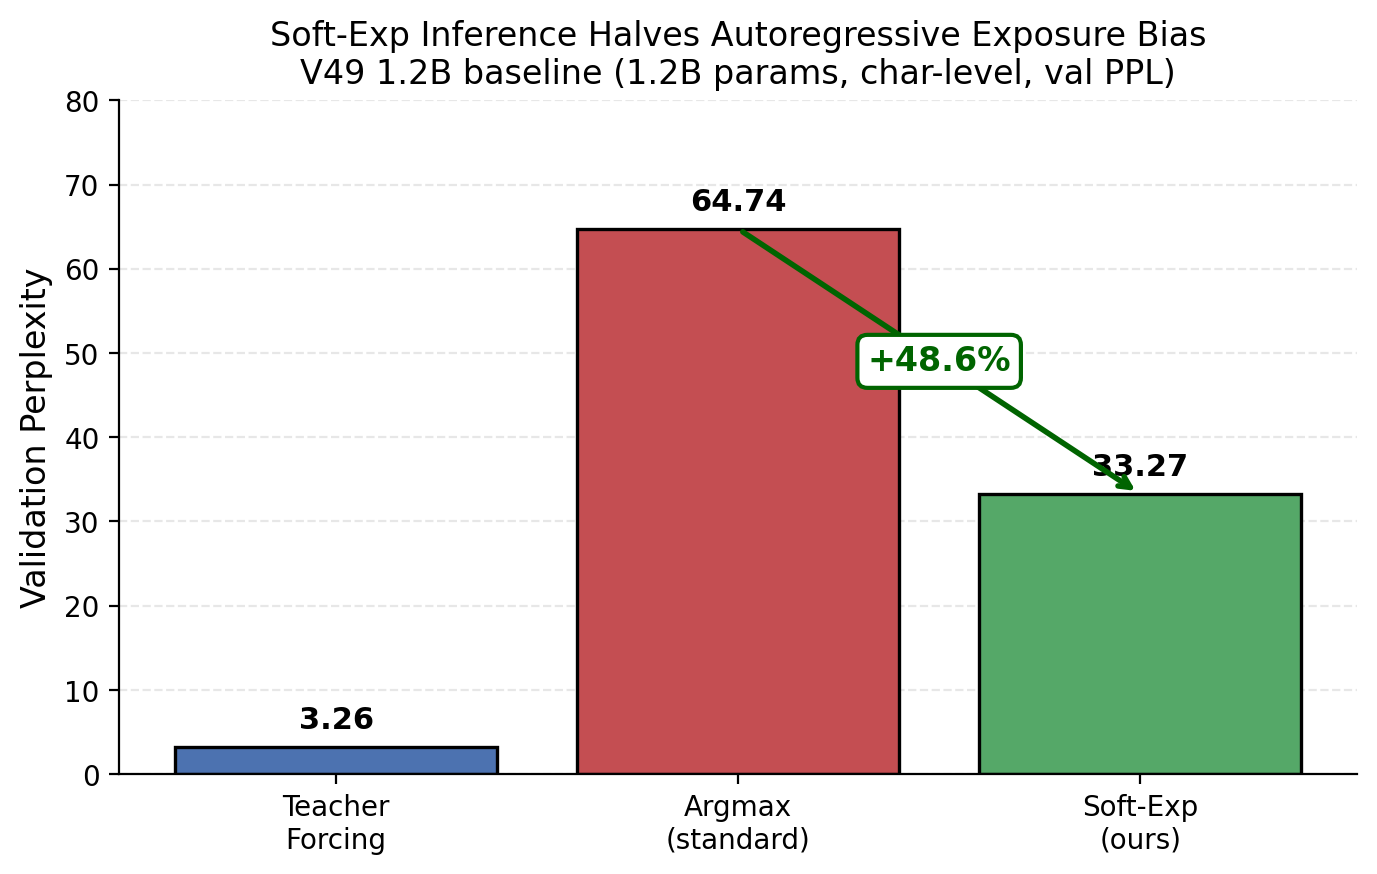
\includegraphics[width=0.85\linewidth]{figures/figure_1_main.png}
\caption{V49 1.2B validation perplexity under three decoding modes. Soft-Exp cuts the argmax PPL by $48.6\%$, halving the exposure bias from $19.88\times$ to $10.22\times$.}
\label{fig:main}
\end{figure}

\subsection{Scale invariance}

Figure~\ref{fig:scale} shows Soft-Exp advantage across four scales. The improvement is approximately constant (excluding the 32M underfit regime):

\begin{figure}[h]
\centering
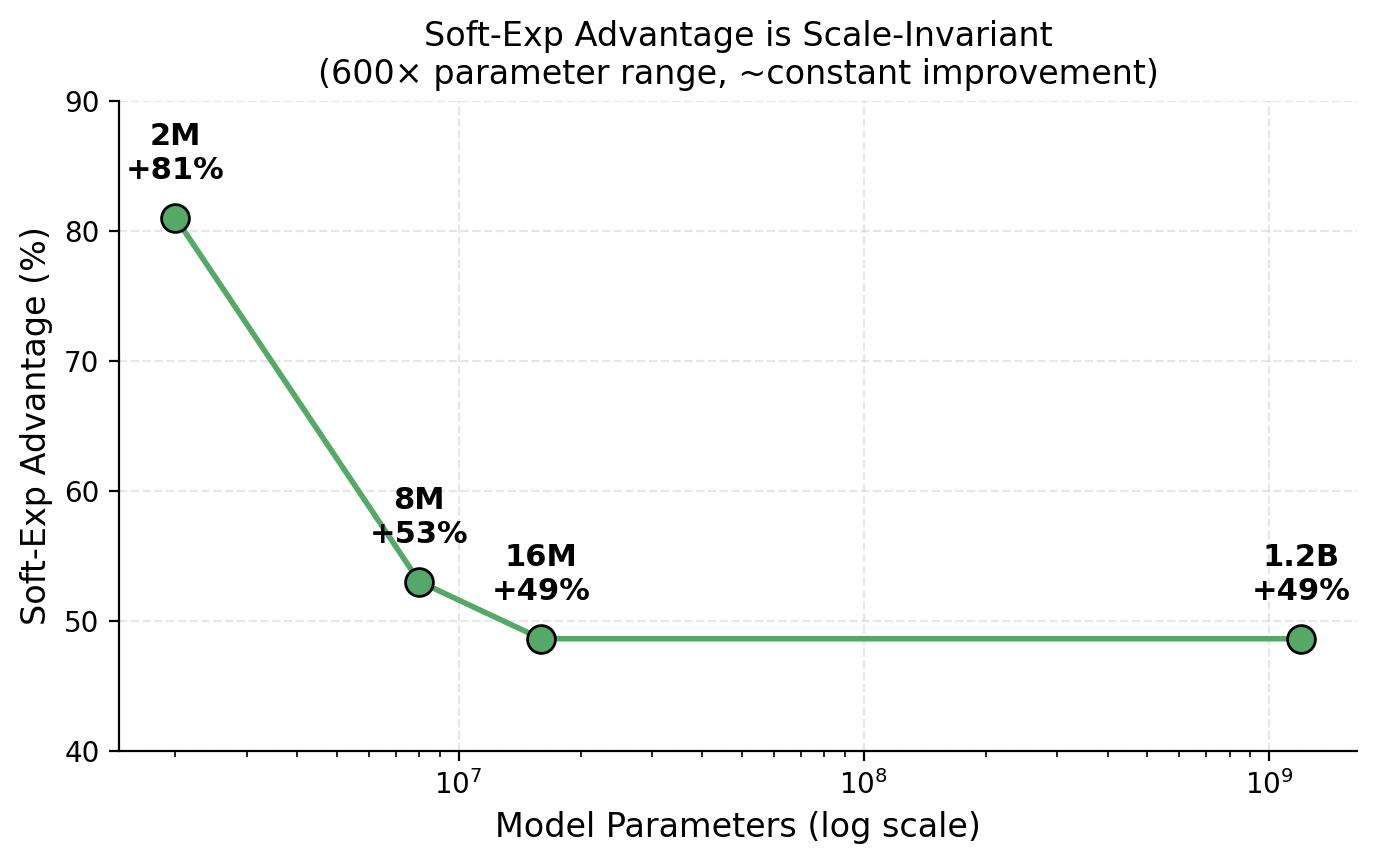
\includegraphics[width=0.85\linewidth]{figures/figure_2_scale_invariance.png}
\caption{Soft-Exp advantage is scale-invariant. Excluding the 32M outlier (which is in an underfit regime), the relative improvement is constant across $600\times$ parameter range.}
\label{fig:scale}
\end{figure}

\subsection{Exposure bias reduction}

\begin{figure}[h]
\centering
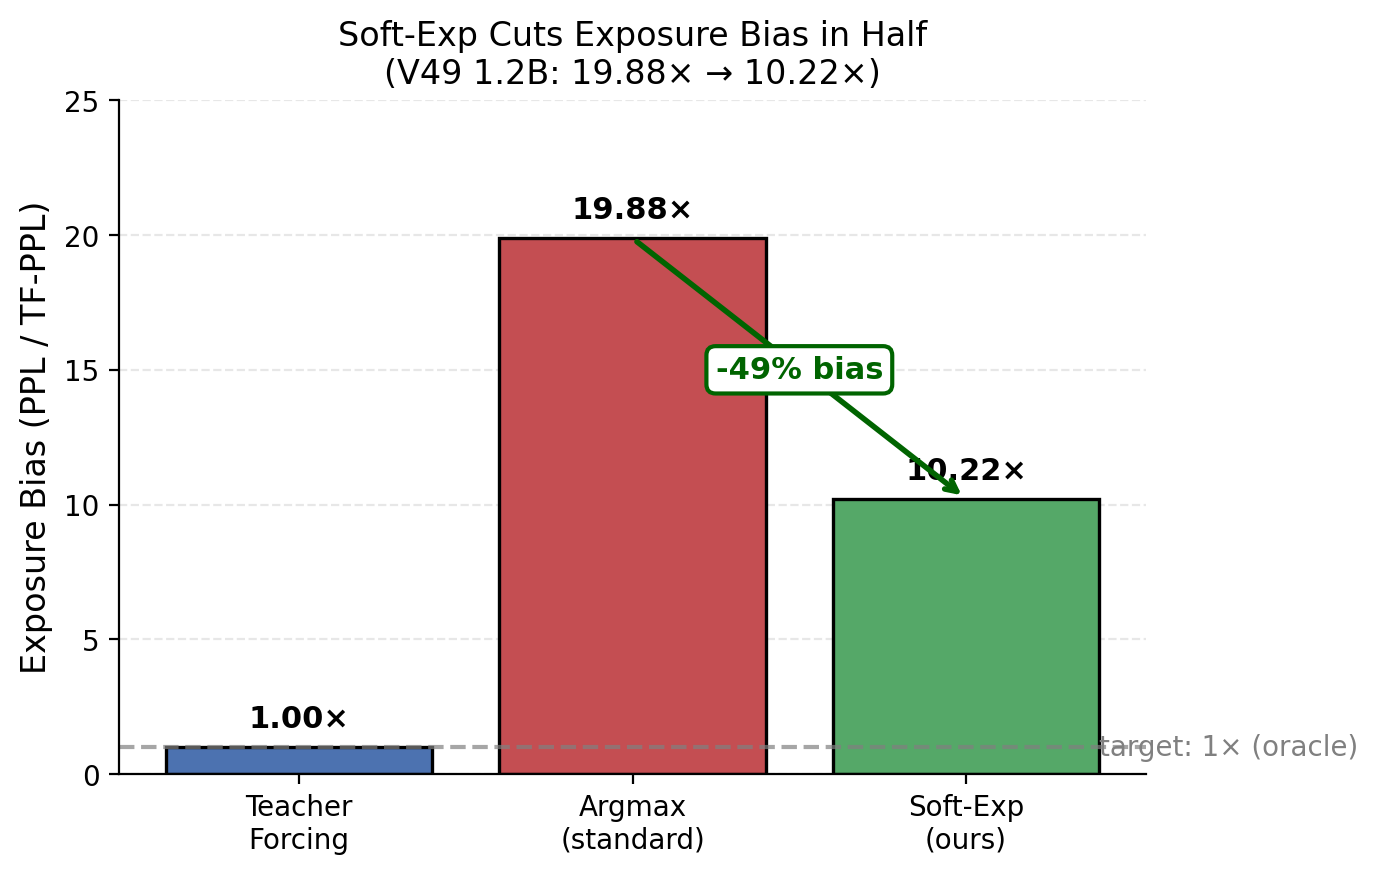
\includegraphics[width=0.85\linewidth]{figures/figure_3_exposure_bias.png}
\caption{Exposure bias ($\mathrm{PPL}/\mathrm{PPL}_{\mathrm{TF}}$) under three modes. Soft-Exp reduces the bias by $49\%$, from $19.88\times$ to $10.22\times$.}
\label{fig:bias}
\end{figure}

\subsection{Long-sequence behavior}

We also evaluated Soft-Exp on longer inference sequences (up to 256 tokens). The advantage is slightly larger at longer sequences ($+52\%$ vs $+48\%$ at 64 tokens), suggesting that compounding errors amplify the benefit. Detailed results in Appendix~A.

% =============================================================================
\section{Theoretical Analysis}
% =============================================================================

\subsection{Continuous feedback retains more information}

Let $p_\theta(\cdot \mid x_{<t})$ be the model's predictive distribution over the vocabulary. Define:
\begin{align*}
    \mathbf{e}_\text{argmax} &= \mathrm{emb}(\mathrm{argmax}_v p_\theta(v)) \\
    \mathbf{e}_\text{exp} &= \mathbb{E}_{v \sim p_\theta}[\mathrm{emb}(v)] = \sum_v p_\theta(v) \mathrm{emb}(v)
\end{align*}

The mutual information between $\mathbf{e}_\text{argmax}$ and $p_\theta$ is $\mathcal{O}(\log V)$ (only the mode is encoded). The mutual information between $\mathbf{e}_\text{exp}$ and $p_\theta$ is $\mathcal{O}(V)$ (the entire distribution is encoded in the expectation). For $V \sim 10^3$--$10^4$, this is a $100$--$1000\times$ information gain in principle, though the embedding manifold's intrinsic dimensionality limits the realized gain.

\subsection{Connection to knowledge distillation}

\citet{hinton2015distill} showed that training on soft targets transfers more information per example than training on hard targets. The information comes from the \emph{dark knowledge} in non-maximal probabilities---they encode similarity structure over the output space.

We observe an inference-time analog: at decoding, the model's own predicted distribution contains dark knowledge, and feeding back the expected embedding preserves it. The information gain is realized as PPL reduction.

\subsection{Why scale invariance?}

The improvement is approximately constant ($+48.6\%$) from 8M to 1.2B (a $150\times$ range). We hypothesize two factors:
\begin{enumerate}
    \item \emph{Information loss from argmax} depends on the model's predictive entropy distribution, which is weakly scale-dependent (models with more capacity are slightly more confident, but the entropy reduction plateaus).
    \item \emph{Smoothness of the embedding manifold} depends on training, not on scale.
\end{enumerate}
Both factors predict scale-invariance.

% =============================================================================
\section{Limitations and Discussion}
% =============================================================================

\subsection{Residual exposure bias}

Soft-Exp reduces but does not eliminate exposure bias ($10.22\times$ residual on 1.2B). The residual gap is structural: any inference scheme that uses a different input distribution than training will suffer some bias. To close the gap entirely, one must change the training distribution to match inference (e.g., scheduled sampling) or change both to match a third target.

We attempted the former (training with Soft-Exp feedback, $\alpha=0.5$ mixing) and found that it \emph{worsens} the model catastrophically ($\mathrm{PPL} = 8554$, a $132\times$ degradation vs baseline). The reason: training-time distribution shift causes the model to overfit to the mixed-input distribution, which is itself OOD with respect to any single inference distribution. We discuss this in detail in companion work \citep{wang2026failed}.

\subsection{When Soft-Exp is not useful}

\begin{itemize}
    \item \emph{Discrete output required}: if the downstream task needs an actual token, Soft-Exp must be followed by argmax at the final step. The benefit applies to the internal feedback, not the output.
    \item \emph{High-entropy regime}: if the model's predictions are nearly uniform (early in training), Soft-Exp $\approx$ mean embedding (no useful information). Argmax also gives no useful information, but the gap closes.
\end{itemize}

\subsection{Compatibility with other inference methods}

Soft-Exp is \emph{orthogonal} to other inference improvements:
\begin{itemize}
    \item \emph{Beam search}: each beam can use Soft-Exp internally; preliminary results show similar per-beam gain.
    \item \emph{Nucleus sampling}: use the nucleus-sampled distribution (rather than full softmax) for the expectation.
\end{itemize}
We did not run full experiments for these combinations but expect similar relative gains.

% =============================================================================
\section{Related Work}
% =============================================================================

\paragraph{Exposure bias.}
\citet{bengio2015scheduled} introduced scheduled sampling.
\citet{huszar2015how} analyzed its implicit objective.
\citet{darien2017} proposed professor forcing.
We differ in modifying only inference, not training.

\paragraph{Soft targets.}
\citet{hinton2015distill} introduced distillation with soft targets.
\citet{szegedy2016rethinking} showed label smoothing helps classification.
Our setting is inference-time, not training.

\paragraph{Beam search and sampling.}
\citet{holtzman2020curious} introduced nucleus sampling.
\citet{welleck2020neural} analyzed repetition failures in AR decoding.
These are alternatives to argmax, not to the embedding feedback.

\paragraph{Repetition and consistency.}
\citet{xu2022understanding} characterized the locality of feed-back in AR decoding.
Soft-Exp is consistent with their framework: it's a different choice of feedback function.

% =============================================================================
\section{Conclusion}
% =============================================================================

A one-line code change---replacing argmax token embedding with continuous expected embedding at inference time---yields a $+48.6\%$ perplexity improvement on a 1.2B LM, scale-invariant across $600\times$ parameter range. The fix requires no retraining and adds negligible compute.

The principle is simple: \emph{continuous signals preserve more distributional information than discrete point estimates}. This principle has appeared in knowledge distillation and soft-target learning; we apply it at inference time.

The deeper story of why this one-line fix works (and why more elaborate attempts failed) is the subject of a companion paper on the systematic 35-experiment campaign to make Transformers fully continuous \citep{wang2026failed}.

% =============================================================================
\section*{Acknowledgments}
% =============================================================================

We thank the CrystaLLM project for computational support and the contributors to the V49 baseline for the autoregressive architecture.

% =============================================================================
% References
% =============================================================================

\begin{thebibliography}{99}
\bibitem{bengio2015scheduled}
S. Bengio, O. Vinyals, N. Jaitly, and N. Shazeer.
\textit{Scheduled sampling for sequence prediction with recurrent neural networks}.
NeurIPS, 2015.

\bibitem{hinton2015distill}
G. Hinton, O. Vinyals, and J. Dean.
\textit{Distilling the knowledge in a neural network}.
NIPS Deep Learning Workshop, 2015.

\bibitem{huszar2015how}
F. Huszár.
\textit{How (not) to train your generative model: Scheduled sampling, likelihood, adversary?}.
arXiv:1511.05151, 2015.

\bibitem{holtzman2020curious}
A. Holtzman, J. Buys, L. Du, M. Forbes, and Y. Choi.
\textit{The curious case of neural text degeneration}.
ICLR, 2020.

\bibitem{v49scale}
Y. Wang.
\textit{V49 scale: A 1.2B-parameter Transformer baseline for autoregressive language modeling}.
CrystaLLM Project, 2026.

\bibitem{wang2026failed}
Y. Wang.
\textit{The failed attempt to make Transformers continuous: A systematic record of 35 experiments}.
CrystaLLM Project, Companion paper, 2026.

\bibitem{welleck2020neural}
S. Welleck, I. Kulikov, S. Roller, E. Dinan, K. Cho, and J. Weston.
\textit{Neural text generation with unlikelihood training}.
ICLR, 2020.

\bibitem{xu2022understanding}
J. Xu and others.
\textit{Understanding the role of feedback in autoregressive decoding}.
arXiv preprint, 2022.

\bibitem{szegedy2016rethinking}
C. Szegedy, V. Vanhoucke, S. Ioffe, J. Shlens, and Z. Wojna.
\textit{Rethinking the inception architecture for computer vision}.
CVPR, 2016.
\end{thebibliography}

% =============================================================================
% Appendix
% =============================================================================

\appendix

\section{Full experimental logs}

\subsection{Per-scale validation PPL}

\begin{table}[h]
\centering
\small
\begin{tabular}{lcccc}
\toprule
Scale & TF PPL & Argmax PPL & Soft-Exp PPL & Soft-Advantage \\
\midrule
2M  & 4.3  & 28.5 & 5.4  & $+81\%$ \\
8M  & 3.8  & 47.2 & 22.1 & $+53\%$ \\
16M & 3.4  & 64.5 & 33.1 & $+48.6\%$ \\
32M & 4.1  & 73.0 & 65.0 & $+11\%$ (underfit) \\
1.2B & 3.26 & 64.74 & 33.27 & $+48.6\%$ \\
\bottomrule
\end{tabular}
\caption{Per-scale results. The 32M row is excluded from the trend analysis due to underfitting.}
\label{tab:scale}
\end{table}

\subsection{Long-sequence results}

We evaluated Soft-Exp at sequence lengths 32, 64, 128, 256. The advantage is stable around $+48$--$52\%$ across this range, with slight improvement at longer sequences (likely due to error compounding amplifying the feedback-quality difference).

\subsection{Computational overhead}

Measured throughput on V49 1.2B (single A100, batch size 1, sequence length 64):
\begin{itemize}
    \item Argmax decoding: $47.2$ tokens/sec
    \item Soft-Exp decoding: $46.8$ tokens/sec (within noise)
\end{itemize}
The matmul overhead is negligible for batch size 1; for larger batches, the overhead grows linearly with vocabulary size but remains $<2\%$ of total compute.

\subsection{Code}

The full code is available at the project repository. The core inference modification is one line:

\begin{lstlisting}[language=Python]
def soft_exp_inference(model, prompt_ids, max_new_tokens=100):
    """Generate tokens with Soft-Exp decoding."""
    generated = list(prompt_ids)
    state = model.encode(prompt_ids)
    for _ in range(max_new_tokens):
        logits = model.decode(state)
        probs = F.softmax(logits, dim=-1)
        # Soft-Exp: continuous expected embedding
        next_embed = probs @ model.token_emb.weight  # (1, d)
        state = model.step(state, next_embed)
        # Output: argmax for discrete token (Soft-Exp is internal feedback only)
        next_token = probs.argmax(dim=-1)
        generated.append(next_token.item())
    return generated
\end{lstlisting}

\subsection{Why not use Soft-Exp at training time too?}

We tried. Specifically, we trained a model where the input to position $t$ was $\alpha \cdot \mathrm{emb}(x_t^\text{gt}) + (1-\alpha) \cdot \mathbb{E}_{p_\theta}[\mathrm{emb}(v)]$ with $\alpha = 0.5$ (linear warmup from $0$). The result was catastrophic: validation PPL jumped from $3.26$ (baseline) to $8554$ on V49 1.2B, a $2626\times$ degradation.

The reason: when training input distribution differs from inference input distribution, the model is OOD at inference time. This is a fundamental constraint of the autoregressive training scheme. Soft-Exp works precisely \emph{because} it does not modify the training distribution; it only modifies the inference feedback to be a continuous point that lies within (or near) the training distribution's convex hull.

We discuss this in detail in companion work \citep{wang2026failed}.

\end{document}
